\documentclass[]{article}
\usepackage[utf8]{inputenc}
\usepackage[ngerman]{babel}
\usepackage[T1]{fontenc}
\usepackage{%
	ngerman,
	ae,
	times,  %% hier kann man die Schriftart einstellen
	graphicx,
	url,
	scrlayer-scrpage,
	lastpage,
	mathtools,
	geometry,
	multicol,
	cancel,
	xcolor,
	nicematrix,
	xfrac,
	tikz,
	pgfplots,
	amsmath,
	colortbl,
	centernot,
	dsfont,
	textgreek,
	icomma}
\usepackage[thinlines]{easybmat}
\usetikzlibrary{datavisualization}
\usetikzlibrary{datavisualization.formats.functions}
\usetikzlibrary{intersections}
\pgfplotsset{compat=1.17}
\newcommand{\del}[1]{\cancel{~#1~}}
\NiceMatrixOptions{ last-col,code-for-last-col = \color{blue}\scriptstyle,light-syntax}
\newlength\dlf
\newcommand\alignedhighlight[3]{
  % #1 = color
  % #2 = before alignment
  % #3 = after alignment
  &
  \begingroup
  \settowidth\dlf{$\displaystyle #2$}
  \addtolength\dlf{\fboxsep+\fboxrule}
  \hspace{-\dlf}
  \fcolorbox{#1}{#1}{$\displaystyle #2 #3$}
  \endgroup
}
\newcommand{\reference}[1]{ \text{\small{\textcolor{blue}{(#1)}}} }

\newcommand{\topic}{Elektrotechnisch-phys. Grundlagen}
\newcommand{\subtopic}{Aufgaben 1.1 - 1.29}
\newcommand{\authors}{Nils Helming}

%Head and Footnotes
\setlength{\headheight}{2.1\baselineskip} %baselineskip = minimum distance bbetween the bottom of one line to another.
\geometry{bottom = 3cm}
\setlength{\headsep}{\baselineskip}
\ihead[\topic\hrule]{\topic\hrule}
\chead[\subtopic\\~]{\subtopic\\~}
\ohead[\authors\\~]{\authors\\~}
\ifoot[~]{~}
\cfoot[~]{~}
\ofoot[Seite \thepage~von \pageref{LastPage}]{Seite \thepage~von \pageref{LastPage}}

%Paragraph spacings
\setlength{\parindent}{0em} %em = with of an 'M'
\setlength{\parskip}{1ex} %ex = height of an 'x'


\newcommand{\V}{\lor}
\newcommand{\A}{\land}
\newcommand{\T}[1]{\overline{#1}}
\newcommand{\eq}{\Leftrightarrow}
\newcommand{\rarr}{\Rightarrow}
\newcommand{\red}[1]{\textcolor{red}{#1}}

\newcommand{\unit}[1]{\text{#1}}
\newcommand{\fracunit}[2]{\frac{\unit{#1}}{\unit{#2}}}
\newcommand{\textsq}[1]{\ensuremath{\text{#1}^2}}
\newcommand{\tdot}{\ensuremath{\cdot}}


\begin{document}
\section*{Aufgabe 1.1}
\fbox{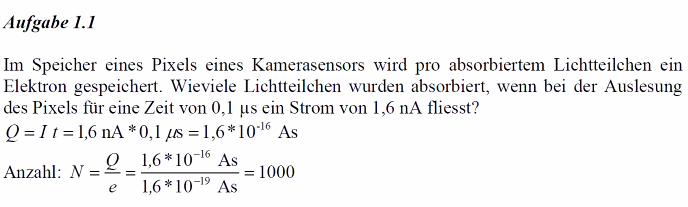
\includegraphics[scale=0.75]{Lösungsbilder/Ueb1_1.png}}\par
	Der Kamerasensor nimmt pro absorbiertem Lichtteilchen ein Elektron auf.
	Es flie"st ein Strom von 1,6nA über eine Zeit von 0,1\textmu s.

	Wie viele Lichtteilchen wurden absorbiert?

	Elementarladung $e = 1,602*10^{-19}$As

	Damit errechnen wir:
	\begin{align*}
	&&	I &= \frac{Q}{t} &&\\
	\text{bzw.}&&  I &= \frac{n \cdot e}{t} &&\\
	\eq&&  n &= \frac{e}{I \cdot t} &&\\
	\text{durch einsetzen von $e$, $I$ und $t$} && n &= \frac{1,602*10^{-19}\unit{As}}{1,6*10^{-9}\unit{A} \cdot 0,1*10^{-6}\unit{s}}&&\\
	&& &= \frac{1,602*10^{-19}\del{\unit{As}}}{0,16*10^{-15}\del{\unit{As}}} &&\\
	&& &= \frac{1,602}{1600} &&\\
	&& &\approx 1000 &&\\
	\end{align*}
\section*{Aufgabe 1.2}
\fbox{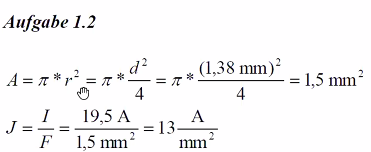
\includegraphics[scale=0.75]{Lösungsbilder/Ueb1_2.png}}\par
	Eine Ader hat einen Durchmesser von $d = 1,38\unit{mm}$.\\ Der maximal erlaubte Strom beträgt $I = 19,5\unit{A}$.

	Damit beträgt die Durchschnittsfläche einer Ader $A = \pi \left(\frac{1,38\unit{mm}}{2}\right)^2 \approx 1,5\unit{mm}^2$

	Und damit die maximale Stromdichte\\
	$ J = \frac{I}{A} = \frac{19,5\unit{A}}{1,5\unit{mm}^2} = 13 \frac{\unit{A}}{\text{mm}^2}$

\section*{Aufgabe 1.3}
\fbox{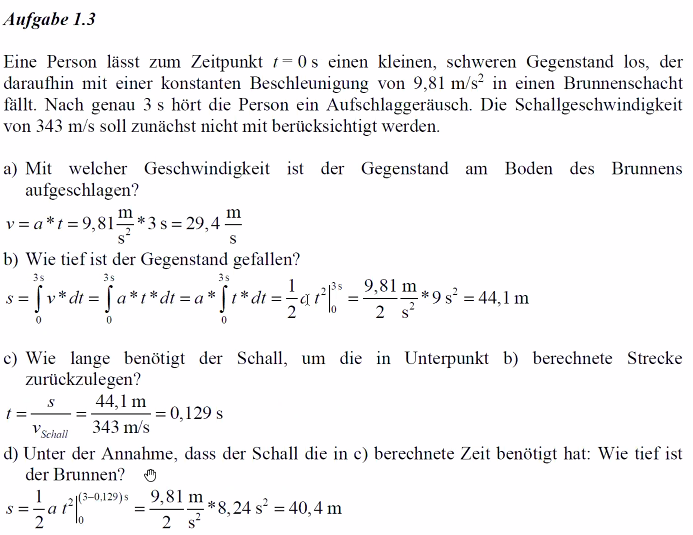
\includegraphics[scale=0.75]{Lösungsbilder/Ueb1_3.png}}\par
\subsection*{(a)}
	Der Gegenstand wurde zum Aufschlagszeitpunt für $t=3\unit{s}$ mit $a=9,81 \unit{m}/\unit{s}^2$ beschleunigt. Das bedeutet mit einer Anfangsgeschwindigkeit von $0\unit{m}/\unit{s}$:\\
	$ v = \int a~dt = \int_{t = 0\unit{s}}^{3\unit{s}}9,81\frac{\unit{m}}{\text{s}^2}~dt = 9,81\frac{\unit{m}}{\text{s}^2} \cdot 3\unit{s} = 29,43\fracunit{m}{s}$
\subsection*{(b)}
	Zuzüglich der Anfangsposition von $0\unit{m}$ ergibt sich:\\
	$ d = \int\int a~dt~dt = \int at~dt = \frac{1}{2}at^2 = \frac{1}{2}9,81\frac{\unit{m}}{\text{s}^2} \cdot (3\unit{s})^2 = 44,145\unit{m}$
\subsection*{(c)}
	Für eine Distanz von $d=44,145\unit{m}$ würde Schall mit einer Geschwindigkeit von $v = 343\fracunit{m}{s}$ die so errechnete Zeit benötigen:\\
	$v = \frac{d}{t} \eq t = \frac{d}{v} = \frac{44,145\unit{m}}{343\fracunit{m}{s}} \approx \frac{1}{8}\unit{s}$
\subsection*{(d)}
	Angenommen das Objekt benötigt $\fracunit{23}{8}\unit{s}$ der $3\unit{s}$ um den Grund des Brunnens zu erreichen, können wir die Rechnung aus (b) wiederholen:\\
	$ d = \frac{1}{2}at^2 = \frac{1}{2}9,81\frac{\unit{m}}{\text{s}^2} \cdot (\fracunit{23}{8}\unit{s})^2 \approx 40,5\unit{m}$

\section*{Aufgabe 1.4}
\fbox{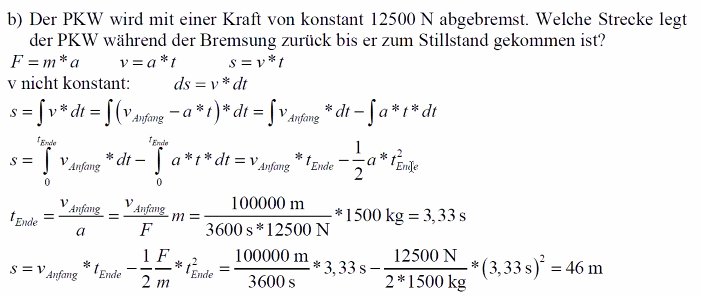
\includegraphics[scale=0.75]{Lösungsbilder/Ueb1_4b.png}}\par
\subsection*{(a)}
	Der PKW fährt mit einer Geschwindigkeit von $100$km/h (ca. $27,8\unit{m/s}$). Somit legt das Fahrzeug $13,9\unit{m}$ innerhalb einer halben Sekunde zurück.
\subsection*{(b)}
	Mit einer Masse von $m = 1500\unit{kg}$ und einer Anfangsgeschwindigkeit von $v_0 = 27,8\unit{m/s}$. Wird der PKW nun mit einer konstanten Kraft $F = 12500\unit{N}$ abgebremst, das bedeutet:\\
	$F = m \cdot a \eq a = \frac{F}{m} = \frac{12500\unit{N}}{1500\unit{kg}} = \frac{25}{3}\fracunit{kg~m}{kg~\textsq{s}} = \frac{25}{3} \fracunit{m}{\textsq{s}}$


	Sei $v(t)$ die Funktion, welche die momentante Geschwindigkeit des PKW während des Bremsprozesses darstellt. Diese ist gegeben durch:\\
	$v(t) = \int -a~dt = -at + v_0 = -\frac{25}{3} \fracunit{m}{\textsq{s}} \cdot t + 27,8\unit{m/s}$\\
	Und $s(t)$ die Funktion, welche die zurückgelegte Strecke seit Beginn des Bremsprozesses angibt:\\
	$s(t)= \int v(t) ~dt = \int -at + v_0~dt = -\frac{1}{2} at^2 + v_0t = -\frac{25}{6}\fracunit{m}{\textsq{s}} \cdot t^2 + 27,8\unit{m/s} \cdot t$


	Gesucht ist der Zeitpunkt zu welchem der PKW $0\unit{m/s}$ erreicht, und die Strecke die zu diesem Zeitpunkt zurückgelegt wurde:
	\begin{flalign*}
		v(t) = 0\unit{m/s} \eq& -\frac{25}{3} \fracunit{m}{\textsq{s}} \cdot t + 27,8\unit{m/s} = 0\unit{m/s} &&\\
		\eq& t = \frac{-27,8\fracunit{m}{s}}{-\frac{25}{3}\fracunit{m}{\textsq{s}}} \approx \frac{10}{3}\unit{s} &&\\
	\end{flalign*}
	$s(\frac{10}{3}\unit{s}) = -\frac{25}{6}\fracunit{m}{\textsq{s}} \cdot (\frac{10}{3}\unit{s})^2 + 27,8\unit{m/s} \cdot \frac{10}{3}\unit{s} = 46,4\unit{m}$

\subsection*{(c)}
	Aus den $13,9\unit{m}$ vor Beginn des Bremsprozesses und den $46,4\unit{m}$ innerhalb dessen ergibt sich eine insgesamt zurückgelegte Strecke von $60,3\unit{m}$.

\subsection*{(d)}
	Mit Änderung der Anfangsgeschwindigkeit auf $v_0 = 130\unit{km/h} \approx 36\unit{m/s}$ legt der PKW in der ersten halben Sekunde also zunächst $18\unit{m}$ zurück und für den Bremsweg ergibt sich:\\
	$v(t) = -\frac{25}{3} \fracunit{m}{\textsq{s}} \cdot t + 36\unit{m/s}$\\
	$s(t) = -\frac{25}{6} \fracunit{m}{\textsq{s}} \cdot t^2 + 36\unit{m/s} \cdot t$\\
	$\Rightarrow t = \frac{-36\fracunit{m}{s}}{-\frac{25}{3}\fracunit{m}{\textsq{s}}} \approx \frac{22}{5}\unit{s}$\\
	$s(\frac{22}{5}\unit{s}) = -\frac{25}{6}\fracunit{m}{\textsq{s}} \cdot (\frac{22}{5}\unit{s})^2 + 36\unit{m/s} \cdot \frac{22}{5}\unit{s} \approx 77,7\unit{m}$\\
	Insgesamt legt der PKW bei einer Anfangsgeschwindigkeit von $130\unit{km/h}$ also $95,7\unit{m}$ zurück.


\section*{Aufgabe 1.5}
\fbox{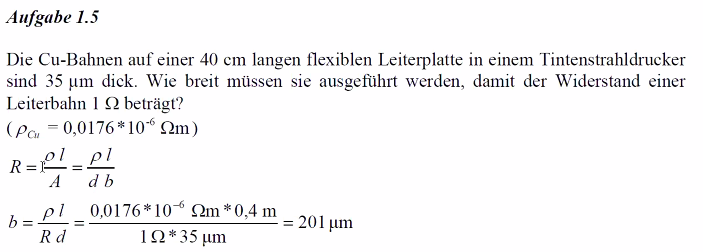
\includegraphics[scale=0.75]{Lösungsbilder/Ueb1_5.png}}\par
	$\rho_{Cu} = 0,0176*10^{-6}\unit{\textOmega m}$\\
	$l = 40\unit{cm} = 0,4\unit{m}$\\
	$A = a \cdot b = 35\unit{\textmu m} \cdot b = 35*10^{-6}\unit{m} \cdot b$\\
	$R = 1\unit{\textOmega} = \frac{\rho \cdot l}{A} = \frac{\rho_{Cu} \cdot l}{a \cdot b}$\\
	$\Rightarrow b = \frac{\rho_{Cu} \cdot l}{a \cdot R} = \frac{0,0176*10^{-6}\unit{\textOmega m} \cdot 0,4\unit{m}}{35*10^{-6}\unit{m} \cdot 1\unit{\textOmega}} = 2,01*10^{-4}\unit{m} = 0,201\unit{mm}$\\

\section*{Aufgabe 1.6}
\fbox{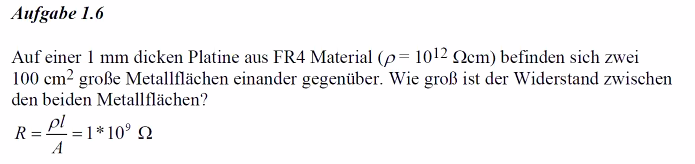
\includegraphics[scale=0.75]{Lösungsbilder/Ueb1_6.png}}\par
	$\rho = 10^{12}\unit{\textOmega cm}$\\
	$l = 1\unit{mm} = 10^{-1}\unit{cm}$\\
	$A = 100\unit{\textsq{cm}}= 10^2\unit{\textsq{cm}}$\\
	$R = \frac{\rho \cdot l}{A} = \frac{10^{12}\unit{\textOmega cm} \cdot 10^{-1}\unit{cm}}{10^2\unit{\textsq{cm}}} = 10^{9}\unit{\textOmega}$

\section*{Aufgabe 1.7}
\fbox{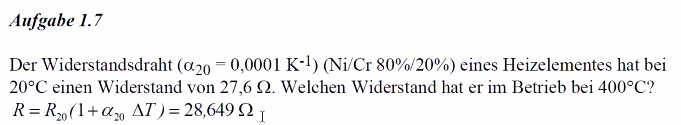
\includegraphics[scale=0.75]{Lösungsbilder/Ueb1_7.png}}\par
	Gegeben ist ein Widerstand ($\alpha_{20} = 0,0001\unit{K}^{-1}$), welcher bei 20°C $R_{20} = 27,6\unit{\textOmega}$ beträgt. Welchen Widerstand hat dieser bei 400°C?\\
	$\Delta T = 400\unit{°C} - 20\unit{°C} = 380 \unit{°C} = 380 \unit{K}$\\
	$R_{400} = R_{20} (1 + \alpha_{20} \cdot \Delta T) = 27,6\unit{\textOmega}(1 + 0,0001\unit{K}^{-1} \cdot 380 \unit{K}) = 27,6\unit{\textOmega}(1,038) \approx 28,65\unit{\textOmega}$

\section*{Aufgabe 1.8}
\fbox{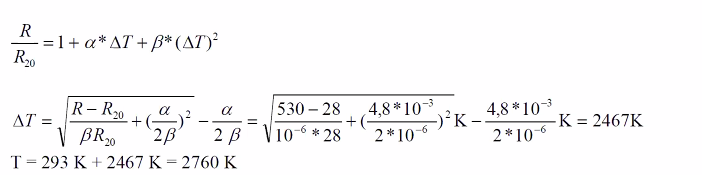
\includegraphics[scale=0.75]{Lösungsbilder/Ueb1_8.png}}\par
\begin{samepage}
	Gegeben ist eine Wolframglühlampe mit folgenden Attributen:\\
	$\alpha = 0,0048\unit{K}^{-1}$\\
	$\beta = 0,000001\unit{K}^{-2}$\\
	$R_{20} = 28 \unit{\textOmega}$\\
	Wie hoch ist die Temperatur des Fadens, wenn dieser einen Wiederstand von $R = 530\unit{\textOmega}$ darstellt?\\
	\begin{align*}
		&& R &= R_{20}(1+ \alpha \cdot \Delta T + \beta \cdot (\Delta T)^2) &&\\
		\eq&& 0 &= R_{20} - R + R_{20} \cdot \alpha \cdot \Delta T + R_{20} \cdot \beta \cdot (\Delta T)^2 &&\\
		&& &= 28 \unit{\textOmega} - 530\unit{\textOmega} + 28 \unit{\textOmega} \cdot 0,0048\unit{K}^{-1} \cdot \Delta T + 28 \unit{\textOmega} \cdot 0,000001\unit{K}^{-2} \cdot (\Delta T)^2 &&\\
		\text{nach pq-Formel}:&& \text{mit~} p &= \frac{28 \unit{\textOmega} \cdot 0,0048\unit{K}^{-1}}{28 \unit{\textOmega} \cdot 0,000001\unit{K}^{-2}} = 4800\unit{K} &&\\
		&& \text{und~} q &= \frac{28 \unit{\textOmega} - 530\unit{\textOmega}}{28 \unit{\textOmega} \cdot 0,000001\unit{K}^{-2}} = \frac{-502}{28}* 10^6 \unit{\textsq{K}} &&\\
		&&\Delta T &= \frac{-4800K}{2} \pm \sqrt{\left(\frac{4800\unit{K}}{2}\right)^2 - \frac{-502}{28}*10^6 \unit{\textsq{K}}} &&\\
		&&\Delta T &= -2400K \pm \sqrt{\frac{161,28}{28}*10^6\unit{\textsq{K}} + \frac{502}{28}* 10^6 \unit{\textsq{K}}} &&\\
		&&\Delta T &= -2400K \pm \sqrt{\frac{663,28}{28}*10^6\unit{\textsq{K}}} &&\\
	\end{align*}
\end{samepage}
\section*{Aufgabe 1.9}
\fbox{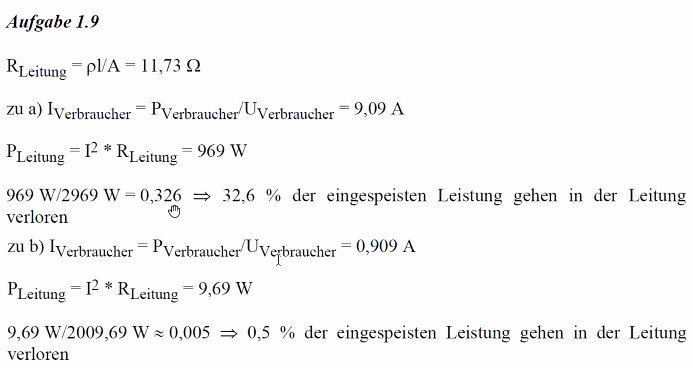
\includegraphics[scale=0.75]{Lösungsbilder/Ueb1_9.png}}\par
	Mit einer Leistungsaufnahme von $P_V = 2000\unit{W}$ bei einer Spannung von $U = 220\unit{V}$, lässt sich mittels $U = R \cdot I$ und $P = U \cdot I$ der Widerstand des Verbrauchers errechnen:\\
	(a) $R_V = \frac{U}{I} = \frac{U^2}{P} = \frac{(220\unit{V})^2}{2000\unit{W}} = 24,2 \fracunit{\textsq{V}}{VA} = 24,2 \unit{\textOmega}$\\
	(b) $R_V = \frac{(2200\unit{V})^2}{2000\unit{W}} = 2420 \unit{\textOmega}$

	Gebündelt haben die beiden Adern eine Länge $l = 1000\unit{m}$, einen Querschnitt von $A = 1,5 \unit{\textsq{mm}} = 1,5 * 10^{-6} \unit{\textsq{m}}$ und einen spezifischen elektrischen Widerstand von $\rho = 0,0176 * 10^{-6}\unit{\textOmega m}$. Somit einen Widerstand von $ R_A = \frac{\rho \cdot l}{A} = \frac{0,0176 * 10^{-6}\unit{\textOmega m} \cdot 1000\unit{m}}{1,5 * 10^{-6} \unit{\textsq{m}}} = 11,7\unit{\textOmega}$

	Also mit $I = \frac{U}{R}$ bilden sich folgende Leistungsaufnahmen:\\
	(a) ohne die Adern: $I_V = \frac{220\unit{A}}{24,2\unit{\textOmega}} = 9,1\unit{A}$\\
	mit den Adern: $I_A = \frac{220\unit{A}}{24,2\unit{\textOmega} + 11,7\unit{\textOmega}} = 6,1\unit{A}$\\
	(b) $I_V$\\

\section*{Aufgabe 1.10}
\fbox{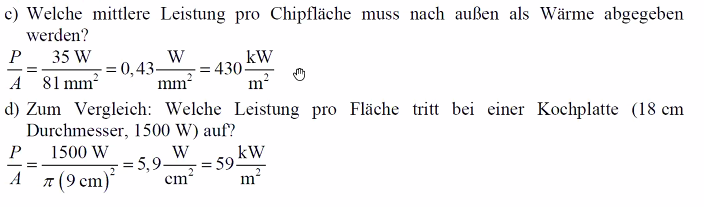
\includegraphics[scale=0.75]{Lösungsbilder/Ueb1_10cd.png}}\par
\subsection*{(a)}
	Angenommen der Stromversorgung ist gleichmäßig auf alle Anschlusskontakte verteilt, können wir annehmen, das $220$ Kontakte benötigt werden, um maximal $I = 55\unit{A}$ versorgen zu können. (für einspeisung und entnahme)
\subsection*{(b)}
	Bei einer Spannung von $U=1,8\unit{V}$ und einer Stromstärke von $55\unit{A}$ würde eine Leistung von $P_{max} = U \cdot I = 1,8\unit{V} \cdot 55\unit{A} = 99\unit{VA} = 99\unit{W}$.
\subsection*{(c)}
	Da jegliche eingespeiste Leisung in Wärme umgewandelt wird, gibt der gesamte Chip eine Wärmeleistung von $P_{avg}=35\unit{W}$ ab, über eine Fläche von $A = 81\unit{\textsq{mm}}$. Also:\\
	$\frac{P_{avg}}{A} = \frac{35\unit{W}}{81\unit{\textsq{mm}}} = \frac{35\unit{W}}{81*10^{-6}\unit{\textsq{m}}} = 0,43*10^{6} \fracunit{W}{\textsq{m}}$
\subsection*{(d)}
	$d = 18\unit{cm}$\\
	$P = 1500\unit{W}$\\
	$A = \pi\cdot (0,5d)^2 = \pi \cdot (9\unit{cm})^2 = \pi \cdot 81\unit{\textsq{cm}} = 254,47*10^{-4}\unit{\textsq{m}}$\\
	$\frac{P}{A} = \frac{1500\unit{W}}{254,47*10^{-4}\unit{\textsq{m}}} = 5,89*10^4 \fracunit{W}{\textsq{m}}$

\section*{Aufgabe 1.11}
\fbox{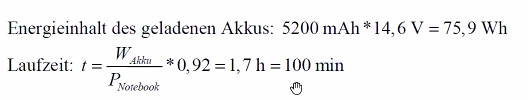
\includegraphics[scale=0.75]{Lösungsbilder/Ueb1_11.png}}\par
	$Q = 5200\unit{mAh}$\\
	$U = 14,6\unit{V}$\\
	$\mu = 92\% = \frac{P_{ab}}{P_{zu}}$\\
	$P_{ab} = 42\unit{W}$ (die an den Laptop abgegebene Leistung)\\
	$P_{zu} = \frac{P_{ab}}{\mu} = 45,65\unit{W}$ (die vom Akkumulator gegebene Leistung)\\
	mit $Q = I \cdot t$ und $P = U \cdot I$ ergibt sich:\\
	$t = \frac{Q}{I} = \frac{Q}{\frac{P}{U}} = \frac{Q \cdot U}{P}$\\
	$t = \frac{5200\unit{mAh} \cdot 14,6\unit{V}}{45,65\unit{W}} = 1663\fracunit{mAh V}{W} = 1663mh = 1,663h$

\section*{Aufgabe 1.12}
\fbox{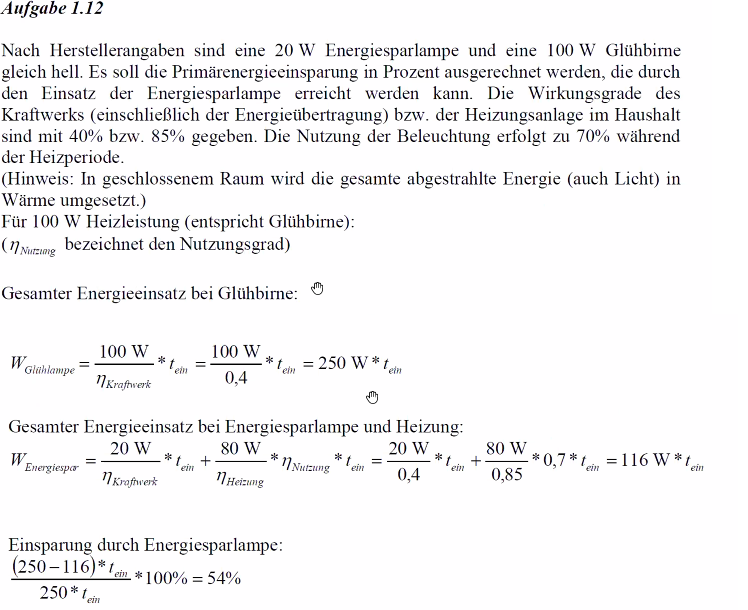
\includegraphics[scale=0.75]{Lösungsbilder/Ueb1_12.png}}\par
	In einem geschlossenen Raum würde jegliche Leistung, die an beide Lampen abgegeben werden in Wärme umgewandelt. Somit produziert die Energiesparlampe eine Wärme von $P_E = 20\unit{W}$ und die Glühlampe $P_G = 100\unit{W}$. Dementsprechend müsste die verlorene Wärmeleistung $P_W = 80\unit{W}$ (nach auswechseln der Glühlampe) durch die Heizungsanlage ersetzt werden. Wir wollen also den Prozentualen

\section*{Aufgabe 1.13}
\fbox{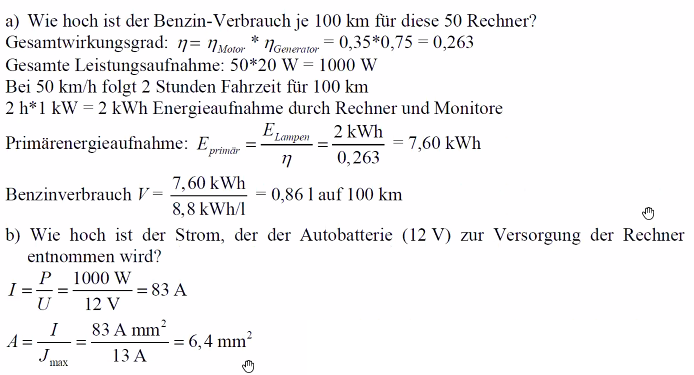
\includegraphics[scale=0.75]{Lösungsbilder/Ueb1_13.png}}\par


\end{document}